\documentclass[crop,tikz,convert={outext=.svg,command=\unexpanded{pdf2svg \infile\space\outfile}},multi=false]{standalone}

\begin{document}
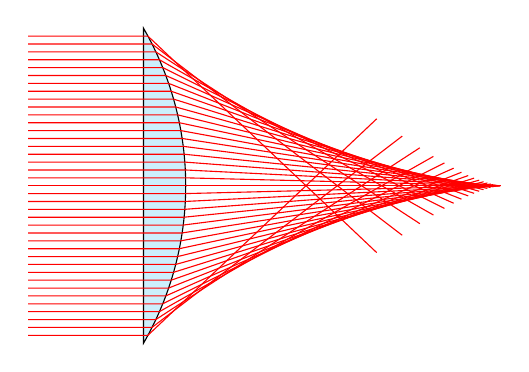
\begin{tikzpicture}
  \pgfmathsetmacro{\radius}{4}
  \pgfmathsetmacro{\refractiveindex}{2}
  \draw[fill=cyan!20] (-30:\radius) arc (-30:30:\radius) -- cycle;
  \foreach \Y in { 0.1,0.2,...,1.9 } {%
    \pgfmathsetmacro{\X}{sqrt(\radius*\radius-\Y*\Y)}
    \draw[red] (2, \Y) -- ({\X}, \Y) -- +({atan( \Y/\X) - asin(\refractiveindex*sin(atan( \Y/\X)))}:4);
    \draw[red] (2,-\Y) -- ({\X},-\Y) -- +({atan(-\Y/\X) - asin(\refractiveindex*sin(atan(-\Y/\X)))}:4);
  }
  \pgfmathsetmacro{\X}{\radius}
  \pgfmathsetmacro{\Y}{0}
  \draw[red] (2, \Y) -- ({\X}, \Y) -- +({atan( \Y/\X) - asin(\refractiveindex*sin(atan( \Y/\X)))}:4);
\end{tikzpicture}
\end{document}
